\subsection{Glyph: \glyph{Necessary stimulation}}
\label{sec:af:necessary_stim}
A \glyph{necessary stimulation} represents that the target activity can only take place if the source activity takes place, regardless of other influences on the target.

\begin{glyphDescription}

\glyphSboTerm SBO:0000171 ! necessary stimulation

  \glyphOrigin One \glyph{biological activity} (\sect{af:biologicalActivity}) or \glyph{logical operator} (\sect{af:logic}).
 \glyphTarget One \glyph{biological activity} (\sect{af:biologicalActivity}) or \glyph{phenotype} (\sect{af:phenotype}).
 \glyphEndPoint The target extremity of a \glyph{necessary stimulation} carries a perpendicular bar followed by an open arrow pointing to the target activity node (\fig{af:trigger}).  The bar must be at least as long as the base of the arrowhead.

\end{glyphDescription}

\begin{figure}[H]
  \centering
  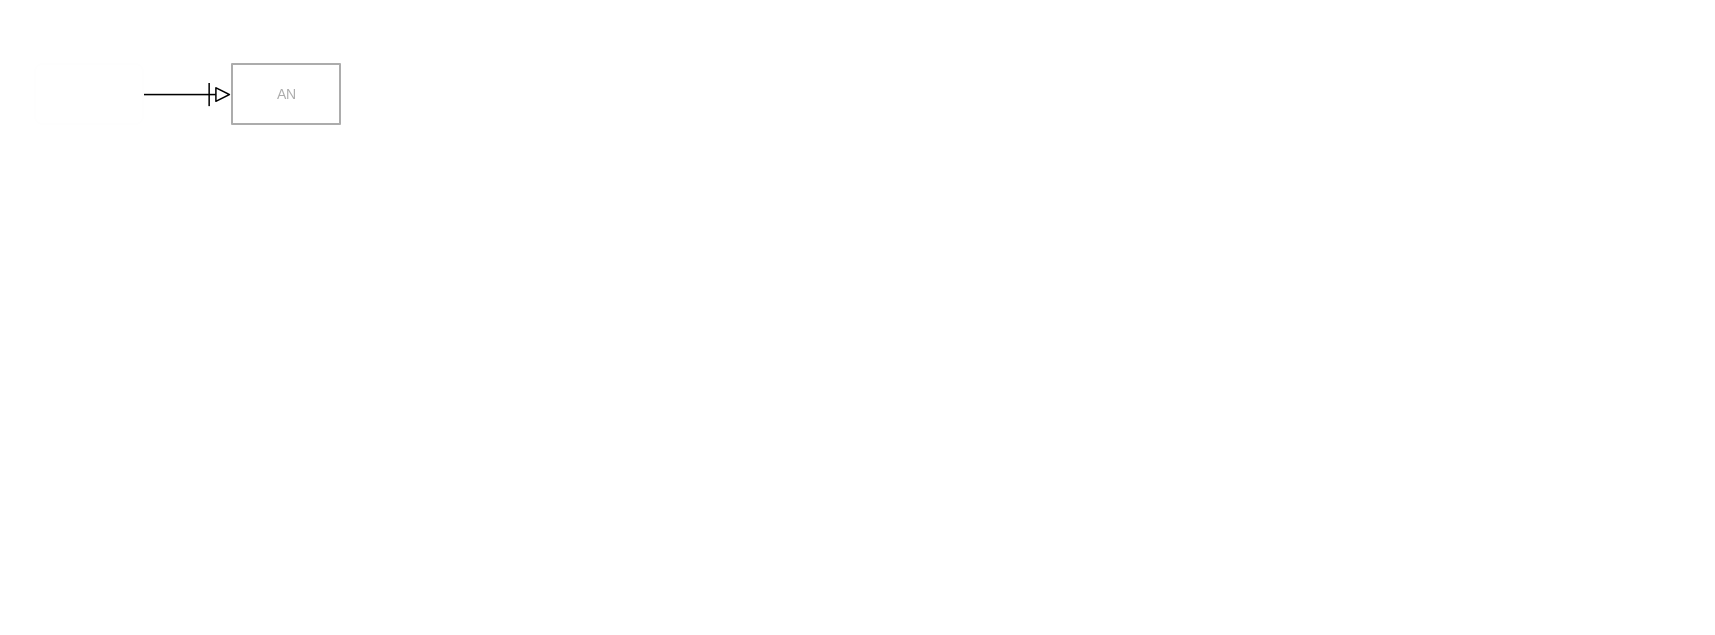
\includegraphics[width = 2in]{images/build/necessary_stimulation.pdf}
  \caption{The \AF glyph for \glyph{necessary stimulation}.}
  \label{fig:af:trigger}
\end{figure}

\begin{figure}[H]
  \centering
  \includegraphics[scale=1]{images/build/necessary_stimulation_example.pdf}
  \caption{An example, taken from \fig{af:1}, of \glyph{necessary stimulation} where nuclear hormone receptor \glyph{PPAR$\delta$} transcription factor activity is necessary for the stimulation of the \glyph{Twist-1} gene expression. }
  \label{fig:af:ex-NS}
\end{figure}
